\chapter{Data Model}\label{ch:datamodel}

\figref{fig:datamodel} shows the analysis classes of the data model used by the
application.

\begin{figure}[htb]
	\includegraphics[width=\textwidth]{datamodel}
	\caption{Data model UML diagram (analysis classes).}\label{fig:datamodel}
\end{figure}

\begin{figure}[htb]
	\centering
	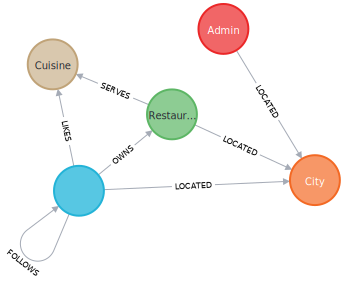
\includegraphics[width=0.6\textwidth]{metagraph}
	\caption{Metagraph with all nodes, labels and
	relationships.}\label{fig:metagraph}
\end{figure}

\begin{figure}[htb]
	\centering
	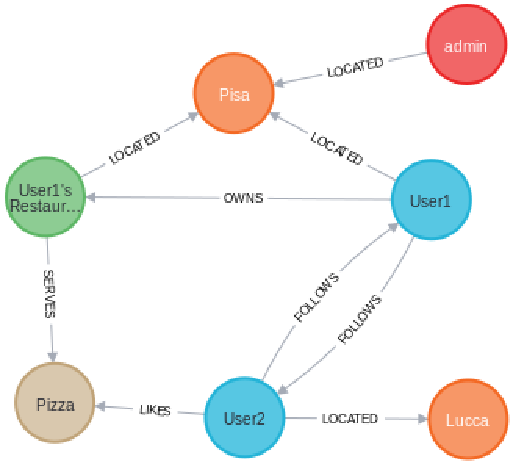
\includegraphics[width=0.6\textwidth]{graph}
	\caption{Graph snapshot (example).}\label{fig:graphsnapshot}
\end{figure}

\figref{fig:metagraph} shows the metagraph of the database. The blue node is a
User node. \figref{fig:graphsnapshot} shows a snapshot of the database.

The following nodes and relations are defined:
\begin{itemize}
	\item[\textbf{User}] \textit{(node)} Represents a user registered in the
		system. It contains the following properties:
		\begin{itemize}
			\item[\textbf{name}] The name of the user, provided
				during registration;
			\item[\textbf{password}] The hash of the password used
				by the user to login.
		\end{itemize}
		Additionally the Administrator has an additional label
		\textbf{Admin} to distinguish him from other regular users.
	\item[\textbf{Restaurant}] \textit{(node)} Represents a restaurant. It
		contains the following properties:
		\begin{itemize}
			\item[\textbf{name}] The name of the restaurant;
			\item[\textbf{price}] An enumerated type that represents
				the expensiveness of the restaurant;
			\item[\textbf{description}] A textual description of the
				restaurant, provided by the restaurant's owner.
		\end{itemize}
	\item[\textbf{City}] \textit{(node)} Represents a city. It contains the
		following properties:
		\begin{itemize}
			\item[\textbf{name}] The name of the city;
			\item[\textbf{latitude}] The latitude, used to compute
				distances;
			\item[\textbf{longitude}] The longitude, used to compute
				distances.
		\end{itemize}
	\item[\textbf{Cuisine}] \textit{(node)} Represents a cuisine type. It
		contains the following properties:
		\begin{itemize}
			\item[\textbf{name}] The cuisine name \exgratia{Pizza}.
		\end{itemize}
	\item[\textbf{OWNS}] \textit{(relation)} Connects a restaurant with his
		owner;
	\item[\textbf{LOCATED}] \textit{(relation)} Connects a user or a
		restaurant with the city where he/she lives in or where it is
		located;
	\item[\textbf{FOLLOWS}] \textit{(relation)} Connects a user with another
		user. A user receives recommendations based on the likes of the
		users he follows;
	\item[\textbf{LIKES}] \textit{(relation)} Connects a user to the
		restaurants/cuisines that he likes;
	\item[\textbf{SERVES}] \textit{(relation)} Connects a restaurant to the
		type of cuisine that it serves.
\end{itemize}

\section{On-Graph Queries}

Four typical ``on-graph'' queries have been defined. The queries allow to
implement the function of restaurant recommendations, user recommendations and
statistics of restaurant of the application on the graph database.

\subsection{Restaurant Recommendations}
\begin{itemize}
	\item [\underline{Domain-Specific}] Find restaurants, which a given user
		has not liked yet, which are located in a given city, or are
		located a given number of kilometers from a given city, which
		make a certain cuisine and which have a certain price.  Sort
		restaurants based on the number of likes of friends, or friends
		of friends, of the given user.
	\item [\underline{Graph-Centric}] Find the restaurant nodes that have a
		\code{LOCATED} relation with a given city or that have a
		\code{LOCATED} relation with a city whose distance from the
		given city is under a given number of kilometers, and have a
		\code{SERVES} relation with a given cuisine and with a given
		value of price attribute. For each resulting restaurant node,
		count the number of \code{LIKES} relation that it has with the
		user nodes that have a \code{FOLLOWS} relation to the given user
		or a \code{FOLLOWS} relation with user nodes that have a
		\code{FOLLOWS} relation with the given user. Sort resulting
		restaurant nodes for the number of \code{LIKES} relation.
\end{itemize}

\subsection{User Recommendations}
\begin{itemize}
	\item [\underline{Domain-Specific}] Find users who are not followed by a
		given user, who lives in a given city, or lives a certain number
		of kilometers away from a given city, who likes a certain
		cuisine. Sort users by distance from the given city.
	\item [\underline{Graph-Centric}] Find the user nodes that have a
		\code{LOCATED} relation with a given city or that have a
		\code{LOCATED} relation with a city whose distance from the
		given city is under a given number of kilometers, and have a
		\code{LIKES} relation with a given cuisine and the given user
		does not have a \code{FOLLOWS} relation with them. Sort
		resulting user nodes by distance with the given city.
\end{itemize}

\subsection{Ranking Restaurant}
\begin{itemize}
	\item [\underline{Domain-Specific}] Given a restaurant, find its
		position in the ranking of restaurants, sorted by the number of
		likes received by users, that are located in the same city, or
		that make the same cuisine of the given restaurant or both.
	\item [\underline{Graph-Centric}] Find restaurant nodes that have a
		\code{LOCATED} relation with the same city node with which the
		given restaurant has a \code{LOCATED} relation or that have a
		\code{SERVES} relation with the same cuisine node with which the
		given restaurant has a \code{SERVES} relation or both of them.
		For each resulting restaurant nodes and for given restaurant,
		count the number of \code{LIKES} relation that it has with user
		nodes. Sort the resulting restaurant nodes for the number of
		\code{LIKES} relation and return the position of the given
		restaurant.
\end{itemize}

\subsection{Likes Restaurant}
\begin{itemize}
	\item [\underline{Domain-Specific}] Find the number of users who have
		liked a certain restaurant.
	\item [\underline{Graph-Centric}] Count the number of user nodes that
		have a \code{LIKES} relation with the specified restaurant.
\end{itemize}
